
\documentclass{beamer}

\mode<presentation>
{
  \usetheme{boxes}
  \usecolortheme[RGB={128,0,0}]{structure}
  \usefonttheme{structurebold}

  \setbeamertemplate{frametitle}[default][center]
  \setbeamertemplate{navigation symbols}{} 
}

\usepackage[english]{babel}
\usepackage[latin1]{inputenc}
\usepackage{times}
\usepackage[T1]{fontenc}
\usepackage{perry-thesis-macros}

\title{Cross-Validation for Principal Components Analysis}

\author[P. O. Perry]{Patrick O. Perry}

\institute[Harvard University]
{
  Statistics and Information Sciences Laboratory\\
  Harvard University
}

\date[BIRS Workshop on Sparse Random Structures]
{January 28, 2010 / BIRS Sparse Random Structures}

\subject{Talks}


\begin{document}

\begin{frame}
  \titlepage
  \hfill\small{(joint work with Art Owen)}
\end{frame}

\section*{Outline}
\begin{frame}
  \frametitle{Outline}
  \tableofcontents
\end{frame}


\section{Introduction}

\subsection{low-rank matrix approximations}
\begin{frame}
\frametitle{Data with large $n$ and $p$}
  \textbf{large number of observations, $n$}

  \textbf{measurements on many variables, $p$} 

  \begin{itemize}
  \item \textit{portfolio selection:} prices of hundreds or thousands of stocks measured every minute 
  \item \textit{genomics:} microarray measurements of thousands or tens-of-thousands of gene expression levels for patients
  \item \textit{text processing:} word frequencies for thousands of words in thousands of documents
  \end{itemize}
\end{frame}

\begin{frame}
\frametitle{Low-rank matrix approximations}
  \centerline{$\mX \approx \mL \mF^\trans$}

  \begin{itemize}
  \item $\mX = \left(\begin{matrix} \vx_1^\trans \\ \vx_2^\trans \\ \vdots \\ \vx_n^\trans \end{matrix} \right) \in \reals^{n \times p}$ is the data matrix
  \item $k \ll \min(n,p)$ is the rank of the approximation
  \item $\mL \in \reals^{n \times k}$ contains factor loadings
  \item $\mF \in \reals^{p \times k}$ contains factors
  \end{itemize}

  \vskip1em
  \textit{Examples:} singular value decomposition, non-negative matrix factorization, $CUR$-decomposition, semi-discrete decomposition, archetypal analysis, \ldots 

  \vskip2em
  \uncover<2->{\centerline{\alert{\Large{How should you pick $k$?}}}}
\end{frame}

\begin{frame}{The singular value decomposition (SVD)}
  \begin{gather*}
    \mX = \sum_{i=1}^{n \wedge p} \sqrt{n} \, \hd_i \vhu_i \vhv_i^\trans = \sqrt{n} \, \mhU \mhD \mhV^\trans \\
    \mhX(k) = \sum_{i=1}^k \sqrt{n} \, \hd_i \vhu_i \vhv_i^\trans = \sqrt{n} \, \mhU \mhD(k) \mhV^\trans
  \end{gather*}

  \begin{itemize}
  \item $\mhU = \left(\begin{matrix} \vhu_1 & \vhu_2 & \cdots & \vhu_{n \wedge p} \end{matrix}\right)$ has orthonormal columns
  \item $\mhV = \left(\begin{matrix} \vhv_1 & \vhv_2 & \cdots & \vhv_{n \wedge p} \end{matrix}\right)$ has orthonormal columns
  \item $\mhD = \diag(\hd_1, \hd_2, \ldots, \hd_{n \wedge p})$ has 
    $\hd_1 \geq \hd_2 \geq \cdots \geq \hd_{n \wedge p} \geq 0$
  \item $\mhD(k) = \diag(\hd_1, \hd_2, \ldots, \hd_k, 0, 0, \ldots, 0)$ 
  \end{itemize}
\end{frame}


\subsection{the latent factor model}

\begin{frame}
\frametitle{When do low-rank approximations make sense?}
  \begin{block}{Data generated by a low-rank process}
    \begin{itemize}
    \item suppose $\vx_i$ is a weighted combination of $k_0$ latent factors corrupted by additive white noise:
      \[ \vx_i = \sum_{j=1}^{k_0} \va_j s_{i,j} + \vepsilon_i = \mA \vs_i + \vepsilon_i \]
    \item $k_0$ is the number of latent factors
    \item $\mA = \left(\begin{matrix} \va_1 & \va_2 & \cdots & \va_{k_0}\end{matrix}\right) \in \reals^{p \times k_0}$ is the matrix of factors
    \item $\vs_i \sim \Normal(0, \mSigma_\text{S}) \in \reals^{k_0}$ is the vector of loadings 
    \item $\vepsilon_i \sim \Normal(0, \sigma^2 \mI) \in \reals^p$ is the noise
    \end{itemize}
  \end{block}
\end{frame}

\begin{frame}
\frametitle{Spiked covariance}
  in the previous model, the covariance of $\vx_i$ is ``spiked'':
  \[
    \mSigma \equiv \E\left[ \vx_i \vx_i^\trans \right] = \mA \mSigma_\text{S} \mA^\trans + \sigma^2 \mI
  \]
  reparametrize:
  \[
    \mSigma = \mQ \mLambda \mQ^\trans + \sigma^2 \mI,
  \]
  where $\mQ$ has orthonormal columns and $\mLambda = \diag( \lambda_1, \lambda_2, \ldots, \lambda_{k_0})$ has $\lambda_1 > \lambda_2 > \cdots > \lambda_{k_0}$
\end{frame}

\begin{frame}
\frametitle{The latent factor model}
  \begin{block}{spiked covariance}
  \[
    \mX \eqd \mZ \mLambda^{1/2} \mQ^\trans + \mE
  \]
  where $Z_{ij} \sim \Normal(0, 1)$, $E_{ij} \sim \Normal(0, \sigma^2)$
  \end{block}
  \begin{block}{general latent factor model}
  \[
    \mX \eqd \sqrt{n} \, \mU \mD \mV^\trans + \mE
  \]
  where
  \begin{itemize}
  \item $\mU = \left(\begin{matrix} \vu_1 & \vu_2 & \cdots & \vu_{k_0}\end{matrix}\right)$
  and $\mV = \left(\begin{matrix} \vv_1 & \vv_2 & \cdots & \vv_{k_0}\end{matrix}\right)$ have orthonormal columns
  \item $\mD = \diag(d_1, d_2, \ldots, d_k)$ has $d_1 > d_2 > \cdots > d_{k_0}$
  \item $E_{ij} \sim \Normal(0, \sigma^2)$
  \end{itemize}
  \end{block}
\end{frame}

\subsection{a loss criterion}

\begin{frame}
  \frametitle{Model error}
  \[
    \ME(k) \equiv \| \sqrt{n} \mU \mD \mV^\trans - \mhX(k) \|_\Frob^2
  \]
  \begin{itemize}
    \item $\mX = \sqrt{n} \mU \mD \mV^\trans + \mE$ is rank-$k_0$ plus noise
    \item $\mX = \sqrt{n} \, \mhU \mhD \mhV^\trans$ is the SVD of $\mX$
    \item $\mhX(k) = \sqrt{n} \, \mhU \mhD(k) \mhV^\trans$ is the rank-$k$ approximation
    \item $\| \cdot \|_\Frob^2$ is squared Frobenius norm (sum of squared elements)
  \end{itemize}
\end{frame}

\begin{frame}
  \frametitle{Prediction error}
  \[
    \PE(k) \equiv \E \| \mX' - \mhX(k) \|_\Frob^2
  \]
  \begin{itemize}
    \item $\mX = \sqrt{n} \mU \mD \mV^\trans + \mE$ is rank-$k_0$ plus noise
    \item $\mX = \sqrt{n} \, \mhU \mhD \mhV^\trans$ is the SVD of $\mX$
    \item $\mhX(k) = \sqrt{n} \, \mhU \mhD(k) \mhV^\trans$ is the rank-$k$ approximation
    \item $\mE' \eqd \mE$ is another realization of the noise
    \item $\mX' = \sqrt{n} \mU \mD \mV^\trans + \mE'$ is another realization of $\mX$
  \end{itemize}
  \vskip1em
  \[
    \PE(k) = \E\left[ \ME(k) \right] + n p \, \sigma^2
  \]
\end{frame}


\section{Behavior of the SVD}

\subsection{sample singular values and vectors}

\begin{frame}
  \frametitle{Asymptotic behavior of singular values}
  \begin{itemize}
  \item assume $n$ and $p$ are both large
  \item $\gamma = \frac{n}{p}$ is the aspect ratio
  \item assume $d_i^2 \toas \mu_i$
  \end{itemize} 
  \begin{theorem}[Onatski, Perry]
    \[
      \hat d_i^2
      \toas
        \begin{cases}
            \left( \mu_i + \sigma^2 \right)
            \left( 1 + \frac{\sigma^2}{\gamma \mu_i} \right)
                &\text{when $\mu_i > \frac{\sigma^2}{\sqrt{\gamma}}$}, \\
            \sigma^2 \left( 1 + \frac{1}{\sqrt{\gamma}} \right)^2
                &\text{otherwise,}
        \end{cases}
    \]
  \end{theorem} 
\end{frame}

\begin{frame}
  \frametitle{Right singular vectors}
  \begin{itemize}
  \item assume $n$ and $p$ are both large
  \item $\gamma = \frac{n}{p}$ is the aspect ratio
  \item assume $d_i^2 \toas \mu_i$
  \end{itemize}
  \begin{theorem}[Onatski, Perry]
    \[
      \mV^\trans \mhV(k)
      \toas
      \diag(\theta_1, \theta_2, \ldots, \theta_k)
    \]
    where
    \[
       \theta_i =  \begin{cases}
            \sqrt{ 
                \left( 1 - \frac{\sigma^4}{ \gamma \mu_i^2} \right) 
                \left( 1 + \frac{\sigma^2}{ \gamma \mu_i  } \right)^{-1} }
            &\text{when $\mu_i > \frac{\sigma^2}{\sqrt{\gamma}}$,} \\
            0
            &\text{otherwise,}
        \end{cases} 
    \]
  \end{theorem}
\end{frame}

\begin{frame} 
  \frametitle{Left singular vectors}
  \begin{itemize}
  \item assume $n$ and $p$ are both large
  \item $\gamma = \frac{n}{p}$ is the aspect ratio
  \item assume $d_i^2 \toas \mu_i$
  \end{itemize}
  \begin{theorem}[Onatski, Perry]
    \[
      \mU^\trans \mhU(k)
      \toas
      \diag(\varphi_1, \varphi_2, \ldots, \varphi_k)
    \]
    where
    \[
      \varphi_i =
        \begin{cases}
            \sqrt{
                \left( 1 - \frac{\sigma^4}{ \gamma \mu_i^2} \right)
                \left( 1 + \frac{\sigma^2}{ \mu_i  } \right)^{-1} }
            &\text{when $\mu_i > \frac{\sigma^2}{\sqrt{\gamma}}$,} \\
            0
            &\text{otherwise,}
        \end{cases}
    \]
  \end{theorem}
\end{frame}

\subsection{loss behavior}

\begin{frame}
  \frametitle{Model error}
  \begin{theorem}
\begin{equation*}
    p \cdot {\ME} (k)
        \toas
        \sum_{i=1}^{k}
            \alpha_i \mu_i
        +
        \sum_{i=k+1}^{k_0}
            \mu_i
        +
        \sigma^2
        \left(
            1 + \frac{1}{\sqrt{\gamma}}
        \right)^2
        \cdot
        (k - k_0)_+,
\end{equation*}
where
\begin{equation*}
    \alpha_i 
    =
    \begin{cases}
        \frac{\sigma^2}{\gamma \mu_i^2}
                \big(
                    3 \sigma^2 + (\gamma+1) \mu_i
                \big)
            &\text{if $\mu_i > \frac{\sigma^2}{\sqrt{\gamma}}$,} \\
        1 
        + 
        \frac{\sigma^2}{\mu_i}
        \left(
            1
            +
            \frac{1}{\sqrt{\gamma}}
        \right)^2
            &\text{otherwise.}
    \end{cases}
\end{equation*}
\end{theorem}
\end{frame}

\begin{frame}
  \frametitle{Frobenius penalty for including $i$th term}
  \begin{center}
  \includegraphics[scale=0.6]{frobenius-loss-penalty}
  \end{center}
\end{frame}

\begin{frame}
  \frametitle{Threshold for inclusion}
  only beneficial to include $i$th term when $\mu_i$ above threshold
  \begin{center}
  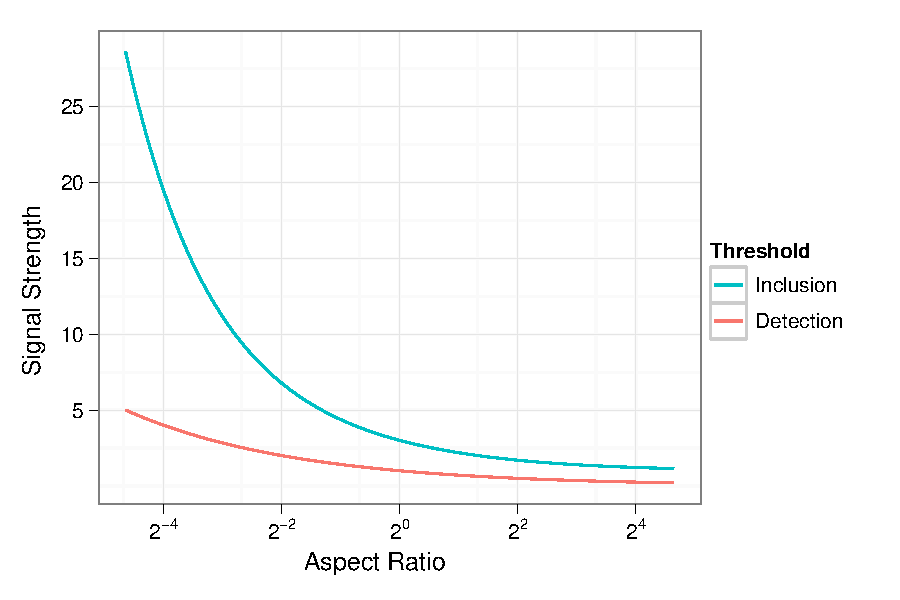
\includegraphics[scale=0.6]{frobenius-loss-cutoff}
  \end{center}
\end{frame}
\subsection{simulations}

\begin{frame}
  \frametitle{Simulation}
  \begin{itemize}
  \item $\gamma = \frac{n}{p} \in \{ 0.25, 1.0, 4.0 \}$
  \item size $n p \in \{ 144, 400, 1600, 4900 \}$
  \item $k_0 = 5$
  \item two components above threshold, two below (one equal)
  \end{itemize}
\end{frame}

\begin{frame}
  \frametitle{Results}
  \begin{center}
  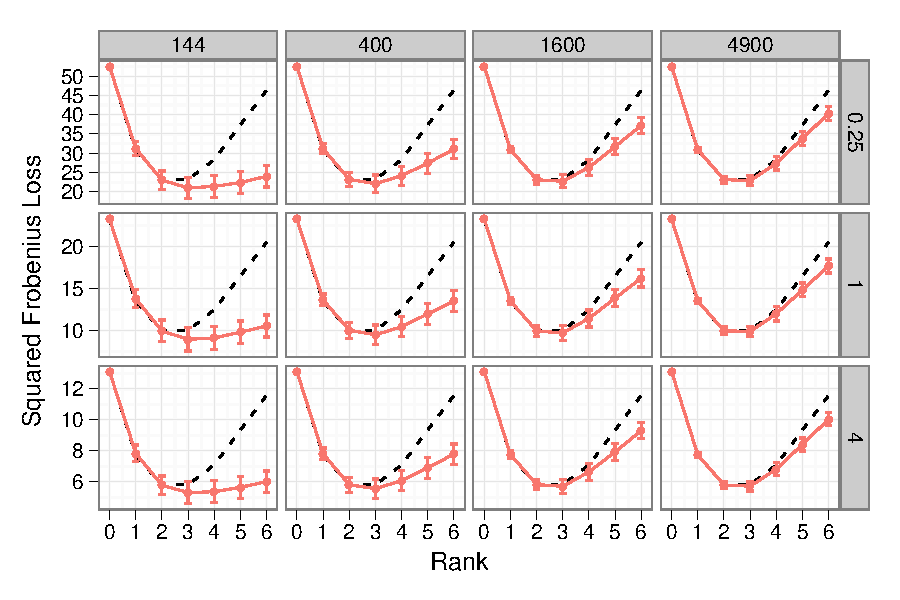
\includegraphics[scale=0.6]{frob2-loss-sim}
  \end{center}
\end{frame}


\section{Cross-validation}

\begin{frame}
  \frametitle{Cross-validation}
  \textbf{use cross-validation (CV) to estimate $\ME(k)$}
  \begin{enumerate}
  \item partition data into \textsc{train} (holdin) and \textsc{test} (holdout) set
  \item fit model to \textsc{train} set   
  \item evaluate performance of model on \textsc{test} set
  \item repeat over many partitions of the data
  \end{enumerate}
\end{frame}

\subsection{Wold-style holdouts}

\begin{frame}
  \frametitle{Wold-style ``speckled'' holdouts}
  \begin{enumerate}
    \item hold out a random subset of elements of $\mX$
    \item fit SVD using expectation-maximizaiton (EM)
    \item evaluate performance
  \end{enumerate}
\end{frame}

\subsection{Gabriel-style holdouts}

\begin{frame}
  \frametitle{Gabriel-style ``blocked'' holdouts}
  \begin{enumerate}
    \item partition
    \(
      \mX = \left(\begin{matrix} \mX_{11} & \mX_{12} \\ \mX_{21} & \ast \end{matrix}\right)
    \)
    \item $\mhU_1 \mhD_1 \mhV_1^\trans$ is the SVD of $\mX_{11}$
    \item $\mhX_{22}(k) = \mX_{21} \mhV_1 \mhD_1(k)^+ \mhU_1^\trans \mX_{12}$ is the prediction of the holdout set
  \end{enumerate}
\end{frame}

\begin{frame}
  \frametitle{Simulations}
  \begin{itemize}
    \item factors $\mU$ and $\mV$ are either ``Gaussian'' or ``sparse''
    \item signal strength $\mD$ is either ``strong'' or ``weak''
    \item black is true model error
    \item red is CV estimate
    \item blue is CV applied to $\mO_L^\trans \mX \mO_R$ (i.e. randomly rotated version of $\mX$) 
  \end{itemize}
\end{frame}

\begin{frame}
  \frametitle{Strong Gaussian factors}
  \begin{center}
  \includegraphics[scale=0.55]{cvsvd-strong-gauss}
  \end{center}
\end{frame}

\begin{frame}
  \frametitle{Strong sparse factors}
  \begin{center}
  \includegraphics[scale=0.55]{cvsvd-strong-sparse}
  \end{center}
\end{frame}
\subsection{theory}

\begin{frame}
  \frametitle{Weak Gaussian factors}
  \begin{center}
  \includegraphics[scale=0.55]{cvsvd-weak-gauss}
  \end{center}
\end{frame}


\begin{frame}
  \frametitle{Weak sparse factors}
  \begin{center}
  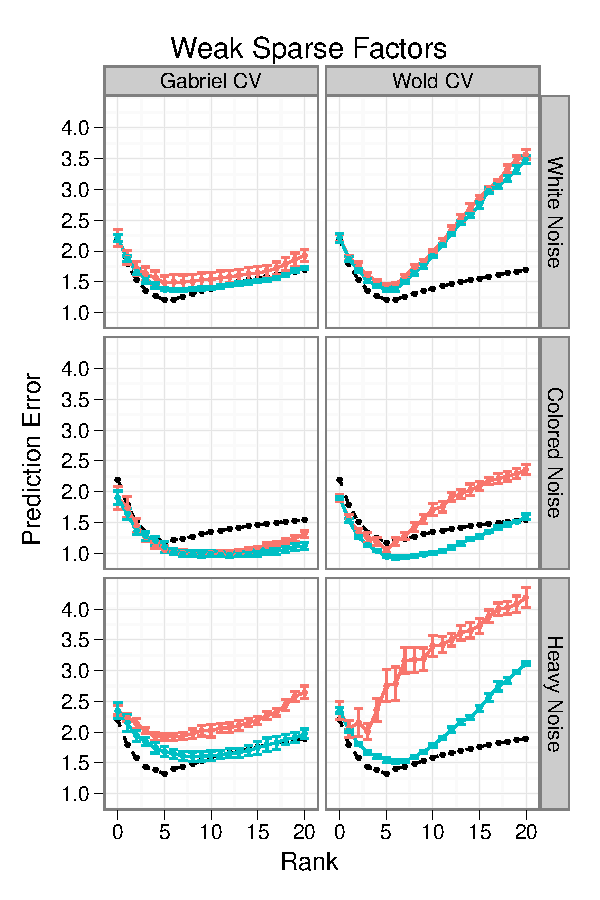
\includegraphics[scale=0.55]{cvsvd-weak-sparse}
  \end{center}
\end{frame}

\begin{frame}
  \frametitle{Theory for Gabriel-style}
  \begin{itemize}
  \item $\hat \sigma^2$ is a $\sqrt{np}$ consistent estimator of $\sigma^2$
  \item technical assumption on factor sparsity
  \end{itemize}
  \begin{theorem}
  \[
\E \left[ p \cdot \widehat{\ME}_n(k) \right]
			\to
				\sum_{i=1}^{k \wedge k_0}
					\beta_i \, \mu_i
				+
				\sum_{i=k+1}^{k_0}
					\mu_i
				+
				\eta
				\cdot
				(k - k_0)_+,
  \]
  where $\beta_i = \ldots$, $\eta_i = \ldots$
  \end{theorem}
\end{frame}

\begin{frame}
  \frametitle{Optimal leave-out size}
  By comparing $\alpha_i$ and $\beta_i$, we determine the optimal leave-out size.
  \begin{theorem}
    If
    \[
       \sqrt{\frac{n_1 p_1}{n p}}
       =
       \frac{\sqrt{2}}{\sqrt{\bar \gamma} + \sqrt{\bar \gamma + 3}}
    \]
    then minimizer of $\E\left[\widehat{ME}(k)\right]$ is same as minimizer of $\ME(k)$;
    here
    \(
      \bar \gamma = (\gamma^{1/2} + \gamma^{-1/2})^2/4
    \),
    $\mX_{11}$ is $n_1 \times p_1$
  \end{theorem}
  (1.89 $\times$ 1.89 is optimal strategy for square matrices)
\end{frame}

\begin{frame}
  \frametitle{Summary}
  \begin{itemize}
    \item model for low-rank plus noise data
    \item asymptotic performance of SVD; sometimes makes sense to include a term, other times not
    \item Wold- and Gabriel-style CV for estimation performance of SVD
    \item theory (optimal holdout) for Gabriel-style CV 
  \end{itemize}
\end{frame}

\end{document}


